\documentclass{article}

\usepackage{fancyhdr}
\usepackage{extramarks}
\usepackage{amsmath}
\usepackage{amsthm}
\usepackage{amsfonts}
\usepackage{tikz}
\usepackage{algorithm}  
\usepackage{algpseudocode}  
\usepackage{amsmath}  
\usepackage{enumerate}
\usepackage{multicol}  
\usepackage{multirow}  
\usepackage{subfigure} 

\usetikzlibrary{automata,positioning}

%
% Basic Document Settings
%  

\topmargin=-0.45in
\evensidemargin=0in
\oddsidemargin=0in
\textwidth=6.5in
\textheight=9.0in
\headsep=0.25in

\linespread{1.1}

\pagestyle{fancy}
\lhead{\hmwkAuthorName}
\chead{\hmwkClass\ (\hmwkClassInstructor): \hmwkTitle}
\rhead{\firstxmark}
\lfoot{\lastxmark}
\cfoot{\thepage}

\renewcommand\headrulewidth{0.4pt}
\renewcommand\footrulewidth{0.4pt}

\setlength\parindent{0pt}

%
% Create Problem Sections
%

\newcommand{\enterProblemHeader}[1]{
    \nobreak\extramarks{}{Problem \arabic{#1} continued on next page\ldots}\nobreak{}
    \nobreak\extramarks{Problem \arabic{#1} (continued)}{Problem \arabic{#1} continued on next page\ldots}\nobreak{}
}

\newcommand{\exitProblemHeader}[1]{
    \nobreak\extramarks{Problem \arabic{#1} (continued)}{Problem \arabic{#1} continued on next page\ldots}\nobreak{}
    \stepcounter{#1}
    \nobreak\extramarks{Problem \arabic{#1}}{}\nobreak{}
}

\setcounter{secnumdepth}{0}
\newcounter{partCounter}
\newcounter{homeworkProblemCounter}
\setcounter{homeworkProblemCounter}{1}
\nobreak\extramarks{Problem \arabic{homeworkProblemCounter}}{}\nobreak{}

%
% Homework Problem Environment
%
% This environment takes an optional argument. When given, it will adjust the
% problem counter. This is useful for when the problems given for your
% assignment aren't sequential. See the last 3 problems of this template for an
% example.
%
\newenvironment{homeworkProblem}[1][-1]{
    \ifnum#1>0
        \setcounter{homeworkProblemCounter}{#1}
    \fi
    \section{Problem \arabic{homeworkProblemCounter}}
    \setcounter{partCounter}{1}
    \enterProblemHeader{homeworkProblemCounter}
}{
    \exitProblemHeader{homeworkProblemCounter}
}

%
% Homework Details
%   - Title
%   - Due date
%   - Class
%   - Section/Time
%   - Instructor
%   - Author
%

\newcommand{\hmwkTitle}{Homework\ \#2}
\newcommand{\hmwkDueDate}{April 7, 2020}
\newcommand{\hmwkClass}{Reinforcement Learning}
\newcommand{\hmwkClassInstructor}{Professor Ziyu Shao}
\newcommand{\hmwkAuthorName}{Tianyuan Wu}
\newcommand{\hmwkAuthorID}{63305667}

%
% Title Page
%

\title{
    \vspace{2in}
    \textmd{\textbf{\hmwkClass:\ \hmwkTitle}}\\
    \normalsize\vspace{0.1in}\small{Due\ on\ \hmwkDueDate\ at 11:59pm}\\
    \vspace{0.1in}\large{\textit{\hmwkClassInstructor}}
    \vspace{3in}
}

\author{\textbf{\hmwkAuthorName}\\ \hmwkAuthorID}
\date{}

\renewcommand{\part}[1]{\textbf{\large Part \Alph{partCounter}}\stepcounter{partCounter}\\}

%
% Various Helper Commands
%

% Useful for algorithms
\newcommand{\alg}[1]{\textsc{\bfseries \footnotesize #1}}

% For derivatives
\newcommand{\deriv}[1]{\frac{\mathrm{d}}{\mathrm{d}x} (#1)}

% For partial derivatives
\newcommand{\pderiv}[2]{\frac{\partial}{\partial #1} (#2)}

% Integral dx
\newcommand{\dx}{\mathrm{d}x}

% Alias for the Solution section header
\newcommand{\solution}{\textbf{\large Solution}}

% Probability commands: Expectation, Variance, Covariance, Bias
\newcommand{\E}{\mathrm{E}}
\newcommand{\Var}{\mathrm{Var}}
\newcommand{\Cov}{\mathrm{Cov}}
\newcommand{\Bias}{\mathrm{Bias}}

\begin{document}

\maketitle

\pagebreak

\begin{homeworkProblem}
    With the same format as bandit algorithms 1,2 and 3, write the pseudo-code of gradient bandit 
    algorithm for this three-armed Bernoulli bandit problem.\\

    \textbf{Solution}
    \begin{algorithm}[h]  
    \caption{Gradient Algorithm}  
    \textbf{Initialize} $\bar{R_t}=0, H(j) = 0, j \in \{1,2,3\}$
        \begin{algorithmic}[1]  
            \For {$t = 1,2,3,\ldots,N$}
                \State $\pi_t(j) \gets \frac{e^{H(j)}}{\sum_{k=1,2,3}{e^{H(k)}}}$, $j \in \{1,2,3\}$
                \State Sample $I(t)$ with probability $P(I(t)=j) = \pi_t(j)$
                \State $\bar{R_t} \gets \frac{1}{t} r_{I(t)} + \frac{t-1}{t} \bar{R_t}$
                \If {Baseline is set}
                    \State $B_t$ $\gets$ Baseline
                \Else
                    \State $B_t$ $\gets$ $\bar{R_t}$
                \EndIf
                \State $H(I(t)) \gets H(I(t)) + \alpha(r_{I(t)}-B_t)(1 - \pi_t(I(t)))$
                \State $H(i) \gets H(i) - \alpha(r_{I(t)}-B_t)\pi_t(i)$, Forall $i \in \{1,2,3\}\ and\ i \neq I(t)$
            \EndFor
        \end{algorithmic}  
    \end{algorithm}  
\end{homeworkProblem}

\begin{homeworkProblem}
    Now suppose we obtain the Bernoulli distribution parameters from an oracle, which are shown in the following 
    table below. Choose $N = 10000$ and compute the theoretically maximized expectation of aggregate rewards over 
    $N$ time slots. We call it the oracle value. Note that these parameters $\theta _j$, $j = 1, 2, 3$ and oracle 
    values are unknown to all bandit algorithms.
    \begin{table}[h]    
        \begin{center}
        \begin{tabular}{|l|l|l|l|}  
        \hline  
        $Arm_j$ & 1&2&3\\
        \hline
        $\theta _j$ & 0.9&0.8&0.7\\
        \hline  
        \end{tabular}  
        \end{center}
    \end{table}

    \textbf{Solution}\\
    We assume $Arm_1$ is chosen $x$ times, $Arm_2$ is chosen $y$ times, then $Arm_3$ is chosen $10000-x-y$ 
    times.
    By the expectation of binomial distribution:
    $$E(X) = np,\ X \sim Bin(n, p)$$
    We can obtain the expectation of aggregate reward $\mathbb{E}_{aggr}$
    $$\mathbb{E}_{aggr} = 0.9x + 0.8y + 0.7(10000-x-y),\ s.t.\ x,y \in \mathbb{N}, x+y \le 10000$$
    Hence, take $x=10000$ and $y=0$, we can get
    \begin{equation}\nonumber
        \begin{aligned}
            \mathbb{E}_{aggr} & = 0.2x + 0.1y + 7000\\
            & \le 2000+0+7000\\
            & = 9000
        \end{aligned}
    \end{equation}
    Thus, if $N=10000$, the theoretically maximized expectation is 9000.
\end{homeworkProblem}

\begin{homeworkProblem}
    Implement classical bandit algorithms\\
    \textbf{Solution}\\
    Codes are in the jupyter-notebook document (.ipynb file).
\end{homeworkProblem}

\begin{homeworkProblem}
    Each experiment lasts for N = 5000 turns, and we run each experiment 1000 times. 
    Results are averaged over these 1000 independent runs.\\
    \textbf{Solution}
    \begin{table}[h]    
        \begin{center}
        \begin{tabular}{|c|c|c|c|c|c|}  
        \hline  
        \multirow{2}{*}{Algorithm} & \multirow{2}{*}{Parameters} & \multicolumn{4}{c|}{Results}\cr
        \cline{3-6} & & $\hat{\theta} _1$ & $\hat{\theta} _2$ & $\hat{\theta} _3$ & Aggregate Reward\\
        \hline  
        $\epsilon$-greedy & $\epsilon=0.1$ & 0.9002 & 0.8008 & 0.7010 & 4446.6\\
        \hline
        $\epsilon$-greedy & $\epsilon=0.5$ & 0.9002 & 0.7995 & 0.7000 & 4248.7\\
        \hline
        $\epsilon$-greedy & $\epsilon=0.9$ & 0.8995 & 0.8005 & 0.6990 & 4047.7\\
        \hline 
        UCB & $c=1$ & 0.9001 & 0.7966 & 0.6921 & 4386.7\\
        \hline
        UCB & $c=5$ & 0.9000 & 0.7997 & 0.6991 & 4124.6\\
        \hline
        UCB & $c=10$ & 0.8999 & 0.7998 & 0.6999 & 4062.8\\
        \hline
        TS  & $\{1,1\}, \{1,1\}, \{1,1\}$ & 0.8998 & 0.7519 & 0.6282 & 4485.1\\
        \hline
        TS  & $\{601,401\}, \{401,601\}, \{2,3\}$ & 0.6835 & 0.4002 & 0.6703 & 3776.2\\
        \hline
        Gradient & baseline=0 & - & - & - & 4425.2\\
        \hline 
        Gradient & baseline=0.8 & - & - & - & 4431.1\\
        \hline 
        Gradient & baseline=5 & - & - & - & 4200.5\\
        \hline 
        Gradient & baseline=20 & - & - & - & 4109.6\\
        \hline 
        Gradient & $\beta=0.2$ & - & - & - & 4256.6\\
        \hline 
        Gradient & $\beta=1$ & - & - & - & 4428.4\\
        \hline 
        Gradient & $\beta=2$ & - & - & - & 4460.1\\
        \hline 
        Gradient & $\beta=5$ & - & - & - & 4481.0\\
        \hline
        Gradient & $\beta = \frac{5(N-t)}{t}$ & - & - & - & 4490.1\\
        \hline
        \end{tabular}  
        \end{center}
    \end{table}
    \\
    For the time-varient algorithm, I take $\beta=\frac{2(N-t)}{t}$. And for all gradient algorithms, I set $\alpha=0.1$.
\end{homeworkProblem}

\pagebreak
\begin{homeworkProblem}
    \textbf{Solution}
    \begin{enumerate}
    \item $\epsilon$-greedy Algorithm\\
    \textbf{Overall Regret}
    \begin{table}[H]
        \caption{$\epsilon$-greedy Algorithm}
    \begin{center}
        \begin{tabular}{c|c|c}
            Parameter & Accmulated Avg. Regret & Total percentage of optimals\\
            \hline
            $\epsilon$=0.9  & 449.916 & 39.94\%\\
            $\epsilon$=0.5  & 250.978 & 66.28\%\\
            $\epsilon$=0.1 &  53.508 & 92.52\%\\
        \end{tabular}
    \end{center}
    \end{table}
    \textbf{Regret-time function}
    \begin{figure}[H]
        \centering
        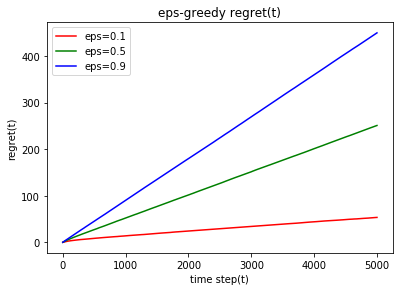
\includegraphics[scale=0.5]{1111.png}
        \caption{$\epsilon$-greedy algorithm: regret-t}
    \end{figure}
    \begin{figure}[H]
        \centering
        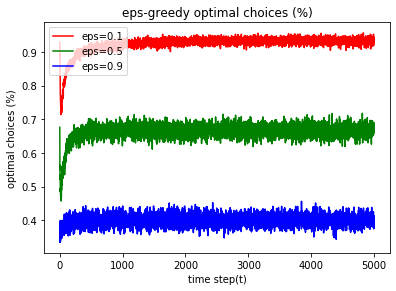
\includegraphics[scale=0.5]{2222.png}
        \caption{$\epsilon$-greedy  algorithm: Percentage of optimals}
    \end{figure}
    \pagebreak

    \item UCB Algorithm\\
    \textbf{Overall Regret}
    \begin{table}[H]
        \caption{UCB Algorithm}
        \begin{center}
        \begin{tabular}{c|c|c}
            Parameter & Accmulated Avg. Regret & Total percentage of optimals\\
            \hline
            c=1   &  114.09 & 82.44\% \\
            c=5   &  374.568 & 47.28\% \\
            c=10  &  437.854 & 40.20\% \\
        \end{tabular}
    \end{center}
    \end{table}
    \textbf{Regret-time function}
    \begin{figure}[H]
        \centering
        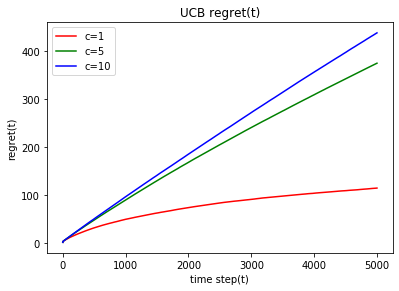
\includegraphics[scale=0.5]{3333.png}
        \caption{UCB algorithm: regret-t}
    \end{figure}
    \begin{figure}[H]
        \centering
        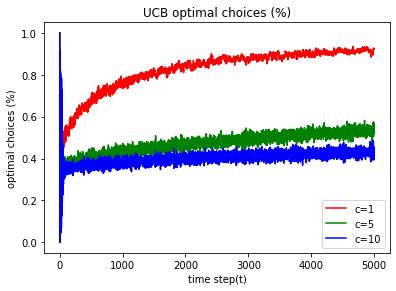
\includegraphics[scale=0.5]{4444.png}
        \caption{UCB algorithm: Percentage of optimals}
    \end{figure}

    \pagebreak
    
    \item TS Algorithm\\
    \textbf{Overall Regret}
    \begin{table}[H]
        \caption{TS Algorithm}
        \begin{center}
        \begin{tabular}{c|c|c}
            Parameter & Accmulated Avg. Regret & Total percentage of optimals\\
            \hline
            \{\{1,1\}, \{1,1\}, \{1,1\}\}  &  15.985 & 97.55\%\\
            \{\{601,401\}, \{401,601\}, \{2,3\}\}  & 723.78 & 28.67\%\\              
        \end{tabular}
    \end{center}
    \end{table}
    \textbf{Regret-time function}
    \begin{figure}[H]
        \centering
        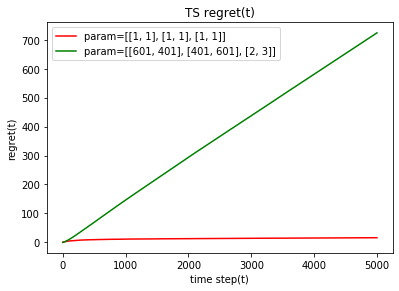
\includegraphics[scale=0.5]{5555.png}
        \caption{TS algorithm: regret-t}
    \end{figure}
    \begin{figure}[H]
        \centering
        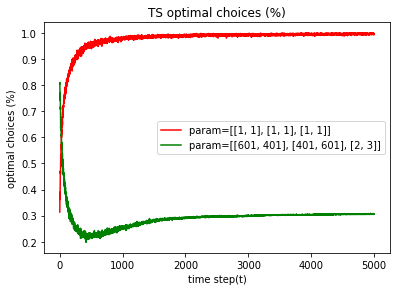
\includegraphics[scale=0.5]{6666.png}
        \caption{TS algorithm: Percentage of optimals}
    \end{figure}

    \pagebreak

    \item Gradient algorithm\\
    \textbf{Overall Regret}
    \begin{table}[H]
        \caption{Gradient Algorithm}
        \begin{center}
        \begin{tabular}{c|c|c}
            Parameter & Accmulated Avg. Regret & Total percentage of optimals\\
            \hline
            baseline=0   &  74.8      & 89.83\% \\
            baseline=0.8 &  68.9      & 90.66\% \\
            baseline=5   &  299.5     & 60.14\% \\
            baseline=20  &  390.4     & 47.98\% \\
            \hline
            $\beta=0.2$  &  243.4     & 71.64\% \\
            $\beta=1$    &  71.6      & 90.62\% \\
            $\beta=2$    &  39.9      & 94.66\% \\
            $\beta=5$    &  19.0      & 97.43\% \\
            \hline 
            time-varient &  9.899     & 98.68\% \\
        \end{tabular}
    \end{center}
    \end{table}
    \textbf{Regret-time function}\\
    \begin{figure}[H]
        \centering
        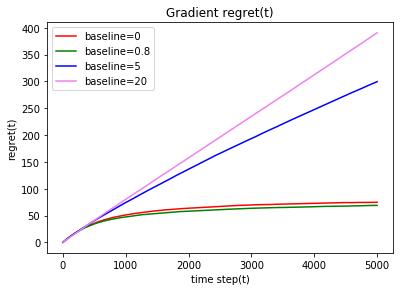
\includegraphics[scale=0.4]{7777.png}
        \caption{Gradient algorithm (baseline): regret-t}
    \end{figure}
    \begin{figure}[H]
        \centering
        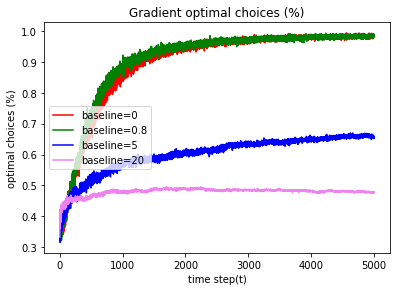
\includegraphics[scale=0.4]{8888.png}
        \caption{Gradient algorithm (baseline): Percentage of optimals}
    \end{figure}

    \begin{figure}[H]
        \centering
        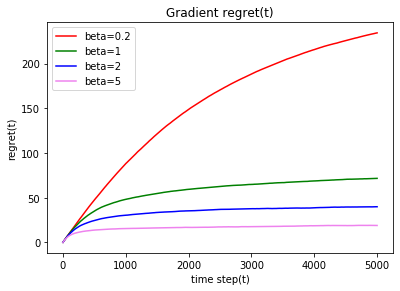
\includegraphics[scale=0.4]{9999.png}
        \caption{Gradient algorithm (parameter): regret-t}
    \end{figure}
    \begin{figure}[H]
        \centering
        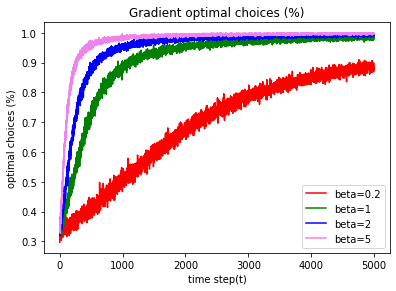
\includegraphics[scale=0.4]{1010.png}
        \caption{Gradient algorithm (parameter): Percentage of optimals}
    \end{figure}

    \begin{figure}[H]
        \centering
        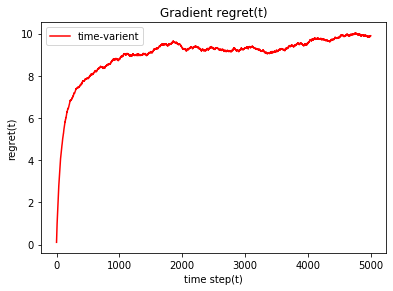
\includegraphics[scale=0.4]{tv1.png}
        \caption{Gradient algorithm (time-varient): regret-t}
    \end{figure}
    \begin{figure}[H]
        \centering
        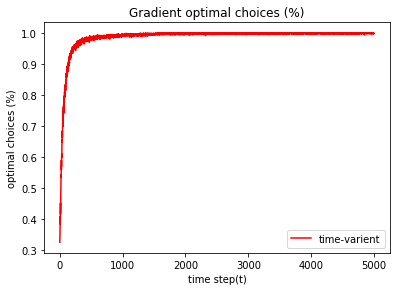
\includegraphics[scale=0.4]{tv2.png}
        \caption{Gradient algorithm (time-varient): Percentage of optimals}
    \end{figure}
    \end{enumerate}
\end{homeworkProblem}


\begin{homeworkProblem}
    \begin{table}[h]    
        \begin{center}
        \begin{tabular}{|c|c|c|}  
        \hline  
        Algorithm & Parameter & Gap\\
        \hline  
        $\epsilon$-greedy & $\epsilon=0.1$ & 53.5\\
        \hline
        $\epsilon$-greedy & $\epsilon=0.5$ & 251.0\\
        \hline
        $\epsilon$-greedy & $\epsilon=0.9$ & 449.9\\
        \hline 
        UCB & $c=1$  & 114.1\\
        \hline
        UCB & $c=5$  & 374.6\\
        \hline
        UCB & $c=10$ & 437.8\\
        \hline
        TS  & $\{1,1\}, \{1,1\}, \{1,1\}$ & 15.9\\
        \hline
        TS  & $\{601,401\}, \{401,601\}, \{2,3\}$ & 723.8\\
        \hline
        Gradient & baseline=0 & 74.8\\
        \hline 
        Gradient & baseline=0.8 & 68.9\\
        \hline 
        Gradient & baseline=5 & 299.5\\
        \hline 
        Gradient & baseline=20 & 390.4\\
        \hline 
        Gradient & $\beta=0.2$ & 243.4\\
        \hline 
        Gradient & $\beta=1$ & 71.6\\
        \hline 
        Gradient & $\beta=2$ & 39.9\\
        \hline 
        Gradient & $\beta=5$ & 19.0\\
        \hline
        Gradient & time-varient & 9.9\\
        \hline
        \end{tabular}  
        \end{center}
    \end{table}
    The results are shown in Table.x, we can obverse that the gradient algorithm with 
    time-varient $\beta$ has the best performance. 
    The impacts are:
    \begin{enumerate}
        \item $\epsilon$-greedy\\
            When $\epsilon$ becomes larger, the exploitation increases, while explanition decreases.\\
            When $\epsilon$ becomes smaller, the exploitation decreases, while explanition increases.\\
            So, during the process that $\epsilon$ increases from a small value to 1, the gap first 
            becomes smaller, then becomes larger.
        \item UCB\\
            When $c$ increases, the gap becomes larger.
        \item TS\\
            When the parameters satisify $\frac{\alpha _i}{\alpha _i + \beta _i} = \theta _i$, the gap reaches the smallest value.
        \item Gradient\\
            When baseline reaches the optimal value (0.9 in this situation), the gap reaches the smallest value.
            Also, during the process that $\beta$ increases from a small value to a large value, the gap first 
            becomes smaller, then becomes larger.
    \end{enumerate}
\end{homeworkProblem}

\pagebreak

\begin{homeworkProblem}
    Give your understanding of the exploration-exploitation trade-off in bandit algorithms.\\
    \textbf{Solution}\\
    Exploration is to ``try something new'', is to explore if there are something better to choose, 
    it may have better rewards, also may have worse rewards. In bandit algorithm, it's to choose 
    a new bandit, it may different from the current optimal one. The algorithm doesn't know it will 
    be better or worse. For example, in $\epsilon$-greedy algorithm, the $\epsilon$ probability is 
    to explore, prevent the algorithm from locking on the local optima. Exploitation is to choose the 
    current optimal bandit based on observations/experiments. It's a greedy choice. So, if we only 
    prefer exploitation, the algorithm will make choice randomly, cannot converge to the optimal value. 
    But if we only consider about exploration, the algorithm may "lock" on some local optimals, cannot 
    find the global optimal solution. Thus, we need to balance exploration and exploitation, try to 
    explore more in the beginning, and then make greedy choices to converge to the optimal value.
\end{homeworkProblem}


\begin{homeworkProblem}
    We implicitly assume the reward distribution of three arms are independent. How about the dependent 
    case? Can you design an algorithm to exploit such information to obtain a better result?\\
    \textbf{Solution}\\
    We can refer to TLP(two-level policy) algorithm, which is introduced in ``multi-armed bandit problems with dependent arms
    - Sandeep Pandey, Deepayan Chakrebarti and Deepak Agarwal, Yahoo! research''. 
    For example, we have 3 arms and a prior that $\theta_1 - \theta_2 \le 0.01$, then we can divide arm 1,2 into 
    cluster1, and arm3 to cluster2. Thus, we can construct a model: $n$ arms are divided into $K$ clusters, 
    by exploiting the dependence information. Then, for each step, we calculate the average reward $\bar{r_k}$ and 
    variance $\sigma(r_k)$ for each cluster. Then call the independent bandit algorithm (e.g. UCB, gradient, etc.) 
    to select a cluster. Then, in the selected group, call independent bandit algorithm again to get a choice. It can 
    be descriped in pseudo-code:
    \begin{algorithm}[h]  
        \caption{TLP Algorithm}  
            \begin{algorithmic}[1]  
                \State Divide $Arm_1, \ldots, Arm_n$ into $K$ clusters $C_1, \ldots, C_K$ by dependence knowledge.
                \For {$t = 1,2,3,\ldots,N$}
                    \State Foreach cluster $C_i$, calculate $\hat{\sigma}_{C_i}(t),\ \hat{r}_{C_i}(t)$.
                    \State Call independent bandit algorithm to choose a cluster $C_t$
                    \State Call independent bandit algorithm in $C_t$, to choose $Arm_t$
                \EndFor
            \end{algorithmic}  
        \end{algorithm} 
\end{homeworkProblem}

\begin{homeworkProblem}
    Please reproduce the proof of regret decomposition lemma.\\
    \textbf{Solution}\\
    For $Q(a_\tau) = \mathbb{E}[r_\tau | a_\tau]$ is a random variable, and by adam's rule,
    $$\mathbb{E}[Q(a_\tau)] = \mathbb{E}[\mathbb{E}[r_\tau | a_\tau]] = \mathbb{E}[r_\tau]$$
    Let $S_t = \sum_{\tau=1}^{t}{Q(a_\tau)}$, then we have:
    $$\mathbb{E}(S_t) = \sum_{\tau=1}^{t}{\mathbb{E}[{Q(a_\tau)}]} = \mathbb{E}[\sum_{\tau=1}^{t}r_\tau]$$
    Since $\sum_{a\in A}1_{a_\tau = a} = 1$ for any fixed $\tau$, then we have:
    \begin{equation}\nonumber
        \begin{aligned}
            \mathbb{E}(S_t) & = \mathbb{E}[\sum_{\tau=1}^{t}r_\tau]\\
            & =  \mathbb{E}[\sum_{\tau=1}^{t}\sum_{a\in A}r_\tau 1_{a_\tau = a}]\\
            & =  \sum_{a\in A}\sum_{\tau=1}^{t}\mathbb{E}[r_\tau 1_{a_\tau = a}]\\
        \end{aligned}
    \end{equation}
    On the other hand, $\sum_{\tau=1}^{t}\sum_{a\in A}1_{a_\tau = a} = t$, so 
    $\sum_{a\in A}\sum_{\tau=1}^{t}\mathbb{E}[1_{a_\tau = a}] = t$.\\
    The total regret can be calculated as:
    \begin{equation}\nonumber
        \begin{aligned}
            L_t & = \mathbb{E}[\sum_{\tau=1}^{t}{V^{*} - Q(a_\tau)}]\\
            & = tv^{*} - \mathbb{E}(\sum_{\tau=1}^{t}Q(a_\tau)) \\
            & = tv^{*} - \mathbb{E}(S_t)\\
            & = tv^{*} - \sum_{a\in A}\sum_{\tau=1}^{t}\mathbb{E}[r_\tau 1_{a_\tau = a}]\\
            & = \sum_{a\in A}\sum_{\tau=1}^{t}\mathbb{E}[1_{a_\tau = a}]v^{*} - \sum_{a\in A}\sum_{\tau=1}^{t}\mathbb{E}[r_\tau 1_{a_\tau = a}]\\
            & = \sum_{a\in A}\sum_{\tau=1}^{t}\mathbb{E}[(v^{*} - r_\tau)1_{a_\tau = a}]
        \end{aligned}
    \end{equation}
    Then, we calculate $\mathbb{E}[(v^{*} - r_\tau)1_{a_\tau = a} | a_\tau]$:
    \begin{equation}\nonumber
        \begin{aligned}
            & \mathbb{E}[(v^{*} - r_\tau)1_{a_\tau = a} | a_\tau] \\
            & = 1_{a_\tau = a}\mathbb{E}[(v^{*} - r_\tau) | a_\tau]\\
            & = 1_{a_\tau = a}(v^{*} - Q(a)) \\
            & = 1_{a_\tau = a}\Delta_a
        \end{aligned}
    \end{equation}
    Thus,
    $$\mathbb{E}[(v^{*} - r_\tau)1_{a_\tau = a}] = \mathbb{E}[1_{a_\tau = a}\Delta_a]$$
    Then we have:
    \begin{equation}\nonumber
        \begin{aligned}
            L_t & = \sum_{a\in A}\sum_{\tau=1}^{t}\mathbb{E}[(v^{*} - r_\tau)1_{a_\tau = a}]\\
            & = \sum_{a\in A}\sum_{\tau=1}^{t}\mathbb{E}[1_{a_\tau = a}\Delta_a]\\
            & = \sum_{a\in A}\mathbb{E}[\sum_{\tau=1}^{t}1_{a_\tau = a}]\Delta_a\\
            & = \sum_{a\in A}\mathbb{E}[N_t(a)]\Delta_a
        \end{aligned}
    \end{equation}
\end{homeworkProblem}

\begin{homeworkProblem}
    Please reproduce the derivation of gradient bandit algorithmem.\\
    \textbf{Solution}\\
    For the gradient ascent algorithm, for each iteration, we have:
    $$w_{t+1} \gets w_t + \nabla_w \mathbb{E}[f(w_t)]$$
    And the objective function is $\max{\mathbb{E}[R_t]}$.
    We have:
    $$\max{\mathbb{E}[R_t]} = \max{\mathbb{E}[\mathbb{E}[R_t|E_t]]} = \sum_x{q_{*}(x)\pi_t(x)}$$
    where $\pi_t(x) = \frac{exp(H_t(x))}{\sum_{y=1}^k{exp(H_t(y))}}$.
    So, $\mathbb{E}[R_t]$ is a function of $H_t(x)$. And for each iteration, we have:
    $$H_{t+1}(a) = H_t(a) +\alpha\frac{\partial \mathbb{E}[R_t]}{\partial H_t(a)}$$
    Then we prove the lemma:
    $$\frac{\partial{\pi(x)}}{\partial{H(a)}} = \pi(x)(1_{\{x=a\}} - \pi(a))$$
    Proof:\\
    \begin{itemize}
        \item {a)} If $x \neq a$: \\
            \begin{equation}\nonumber
                \begin{aligned}
                    \frac{\partial{\pi(x)}}{\partial{H(a)}} & = \frac{\partial{\frac{e^{H(x)}}{\sum_{y=1}^{k}{e^{H(y)}}}}}{\partial{H(a)}}\\
                    & = \frac{0-e^{H(a)}e^{H(x)}}{(\sum_{y=1}^{k}{e^{H(y)}})^2}\\
                    & = - \frac{e^{H(a)}}{\sum_{y=1}^{k}{e^{H(y)}}}\cdot \frac{e^{H(x)}}{\sum_{y=1}^{k}{e^{H(y)}}}\\
                    & = -\pi(a)\pi(x)\\
                    & = \pi(x)(0 - \pi(a))
                \end{aligned}
            \end{equation}
        \item {b)} If $x = a$: \\
        \begin{equation}\nonumber
            \begin{aligned}
                \frac{\partial{\pi(x)}}{\partial{H(a)}} & = \frac{\partial{\frac{e^{H(a)}}{\sum_{y=1}^{k}{e^{H(y)}}}}}{\partial{H(a)}}\\
                & = \frac{e^{H(a)}\cdot \sum_{y=1}^{k}{e^{H(y)}} - (e^{H(a)})^2}{(\sum_{y=1}^{k}{e^{H(y)}})^2}\\
                & = \frac{e^{H(a)}}{\sum_{y=1}^{k}{e^{H(y)}}} \cdot \frac{\sum_{y=1}^{k}{(e^{H(y)})} - e^{H(a)}}{\sum_{y=1}^{k}{e^{H(y)}}}\\
                & = \pi(a)(1 - \pi(a))\\
                & = \pi(x)(1 - \pi(a))
            \end{aligned}
        \end{equation}
    \end{itemize}
    Hence, 
    \begin{equation}\nonumber
        \begin{aligned}
            \frac{\partial{\pi(x)}}{\partial{H(a)}} & = 
            \begin{cases}
                \pi(x)(0 - \pi(a)), x \neq a\\
                \pi(x)(1 - \pi(a)), x = a
            \end{cases}
            \\
            & = \pi(x)(1_{\{x=a\}} - \pi(a))
        \end{aligned}
    \end{equation}
    Hence, 
    $$\frac{\partial \pi_t(A_t)}{\partial H_t(a)} = \pi_t(x)(1_{\{A_t=a\}} - \pi_t(a))$$
    and then:
    $$\frac{\partial \mathbb{E}[R_t]}{\partial H_t(a)} = \sum_x q_{*}(x) \frac{\partial \pi_t(A_t)}{\partial H_t(a)}$$
    Since $\sum_x{\pi_t(x)} = 1$, we have $\sum_x{\frac{\partial \pi_t(A_t)}{\partial H_t(a)}} = 0$.\\
    Thus, we introduce a baseline $B_t$, which is not depend on $x$, satisifies $\sum_x{B_t\frac{\partial \pi_t(A_t)}{\partial H_t(a)}} = 0$.\\
    Then we calculte the partial derivative $\frac{\partial \mathbb{E}(R_t)}{\partial H_t(a)}$
    \begin{equation}\nonumber
        \begin{aligned}
            \frac{\partial \mathbb{E}(R_t)}{\partial H_t(a)} & = \sum_x{(q_{*}(x) - B_t)\frac{\partial \pi_t(A_t)}{\partial H_t(a)}}\\
            & = \sum_x{\pi_t (q_{*}(x) - B_t)\frac{\partial \pi_t(A_t)}{\partial H_t(a)} \frac{1}{\pi_t}}\\
            & = \sum_x{\pi_t (q_{*}(x) - B_t)(1_{x=a} - \pi_t(a))}\\
            & = \mathbb{E}[(q_{*}(x) - B_t) (1_{x=a} - \pi_t(a))]
        \end{aligned}
    \end{equation}
    Now we choose $B_t = \bar{R_t} = \frac{1}{t}\sum_{i=1}^t R_i$.\\
    Then we will show:\\
    $$\mathbb{E}[q_{*}(A_t) (1_{x=a} - \pi_t(a))] = \mathbb{E}[R_t (1_{x=a} - \pi_t(a))]$$
    Proof:\\
    \begin{equation}\nonumber
        \begin{aligned}
            & \mathbb{E}[(q_{*}(A_t)) (1_{x=a} - \pi_t(a))]\\
            & = \mathbb{E}[\mathbb{E}[R_t|A_t]) (1_{A_t=a} - \pi_t(a))]\\
            & = \mathbb{E}[\mathbb{E}[R_t(1_{A_t=a} - \pi_t(a))|A_t] ]\\
            & = \mathbb{E}[R_t(1_{A_t=a} - \pi_t(a))] 
        \end{aligned}
    \end{equation}
    Thus we have:
    $$\frac{\partial \mathbb{E}(R_t)}{\partial H_t(a)} = \mathbb{E}[(q_{*}(A_t) -\bar{R_t}) (1_{A_t=a} - \pi_t(a))] = \mathbb{E}[(R_t-\bar{R_t}) (1_{A_t=a} - \pi_t(a))]$$
    Then, we have the gradient bandit algorithm:
    $$H_{t+1}(a) = H_t(a) +\alpha(R_t-\bar{R_t}) (1_{A_t=a} - \pi_t(a)),\ \forall \alpha \in \{ 1, \ldots, k\}$$ 
    And for the policy gradient, we want to maximize $\mathbb{E}_x[f(x)]$, where $x \sim P_\theta$, $P_\theta$ is the policy, we have:
    \begin{equation}\nonumber
        \begin{aligned}
            \nabla_\theta \mathbb{E}[f(x)] & = \nabla_\theta \sum_x {p(x)f(x)}\\
            & = \sum_x p(x)\frac{\nabla_\theta p(x)}{p(x)} f(x)\\
            & = \sum_x p(x) (\nabla_\theta log(p(x)) f(x))\\
            & = \mathbb{E}[f(x)\nabla_\theta log(p(x))]
        \end{aligned}
    \end{equation}

\end{homeworkProblem}

\end{document}

